\section{\KLUDGE 概要}

\index{Framework}

\begin{figure}[t]
\begin{center}
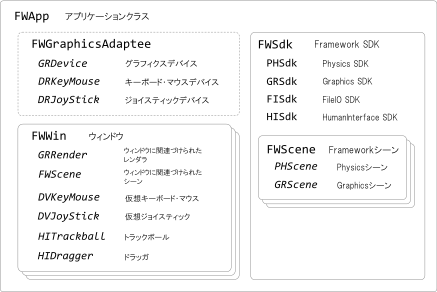
\includegraphics[width=.7\hsize]{fig/framework.eps}
\end{center}
\caption{Framework data structure}
\label{fig_framework}
\end{figure}


Framework\KLUDGE はモジュール間の連携を促進してアプリケーションの作成を支援するためのモジュールです.

Framework\KLUDGE モジュールのデータ構造をFig.\,\ref{fig_framework}\KLUDGE に示します.
\KLUDGE 最上位にはアプリケーションクラス\texttt{FWApp}\KLUDGE があります.
\KLUDGE ユーザは\texttt{FWApp}\KLUDGE を継承することで独自のアプリケーションを作成します.
\texttt{FWApp}\KLUDGE その中にトップレベルウィンドウ(\texttt{FWWin})\KLUDGE の配列,Framework SDK (\texttt{FWSdk})\KLUDGE ,
\KLUDGE およびウィンドウマネジャ(\texttt{FWGraphicsAdaptee})\KLUDGE を持ちます.

\texttt{FWWin}\KLUDGE はトップレベルウィンドウで,そのウィンドウに対応する入力デバイスやビューポート情報を保持するレンダラ,
\KLUDGE そのウィンドウと関連付けられたシーンへの参照などを持ちます.
\KLUDGE また,図中では省略されていますがサブウィンドウやGUI\KLUDGE コントロールを持つこともできます.

\texttt{FWSdk}\KLUDGE の役割は周辺モジュールの機能統合です.
\KLUDGE その中に周辺モジュールのSDK\KLUDGE クラスやFramework\KLUDGE シーン(\texttt{FWScene})\KLUDGE の配列を持ちます.

\KLUDGE ウィンドウマネジャは処理系に依存するデバイスの初期化やイベントハンドリングを行います.
\KLUDGE ウィンドウマネジャはインタフェースを公開していませんのでユーザはその存在を陽に意識する必要はありません.
\KLUDGE 図ではデータ構造の説明のためにあえて記載しています.

\KLUDGE 以下では個々の構成要素について説明していきます.


\section{Framework SDK}

\index{FWSdk}
Framework\KLUDGE モジュールのすべてのオブジェクトはSDK\KLUDGE クラス\texttt{FWSdk}\KLUDGE によって管理されます.
\texttt{FWSdk}\KLUDGE クラスは,プログラムの実行を通してただ1つのオブジェクトが存在するシングルトンクラスです.
\texttt{FWSdk}\KLUDGE オブジェクトを作成するには以下のようにします.
\begin{sourcecode}
FWSdkIf* fwSdk = FWSdkIf::CreateSdk();
\end{sourcecode}
\KLUDGE 通常この操作はプログラムの初期化時に一度だけ実行します.
\texttt{FWSdk}\KLUDGE を作成すると,同時に\texttt{PHSdk}\KLUDGE ,\texttt{GRSdk}\KLUDGE ,\texttt{FISdk}\KLUDGE ,\texttt{HISdk}\KLUDGE も作成されます.
\KLUDGE したがってこれらをユーザが手動で作成する必要はありません.
\KLUDGE 各モジュールの機能にアクセスするには以下の関数によりSDK\KLUDGE を取得します.

\noindent
\begin{tabular}{p{1.0\hsize}}
\\
\texttt{FWSdkIf}				\\ \midrule
\texttt{PHSdkIf* GetPHSdk()}	\\
Physics SDK\KLUDGE を取得する.			\\
\\
\texttt{GRSdkIf* GetGRSdk()}	\\
Graphics SDK\KLUDGE を取得する.		\\
\\
\texttt{FISdkIf* GetFISdk()}	\\
FileIO SDK\KLUDGE を取得する.			\\
\\
\texttt{HISdkIf* GetHISdk()}	\\
HumanInterface SDK\KLUDGE を取得する.	\\
\\
\end{tabular}

\section{Framework \KLUDGE シーン}

\begin{figure}[t]
\begin{center}
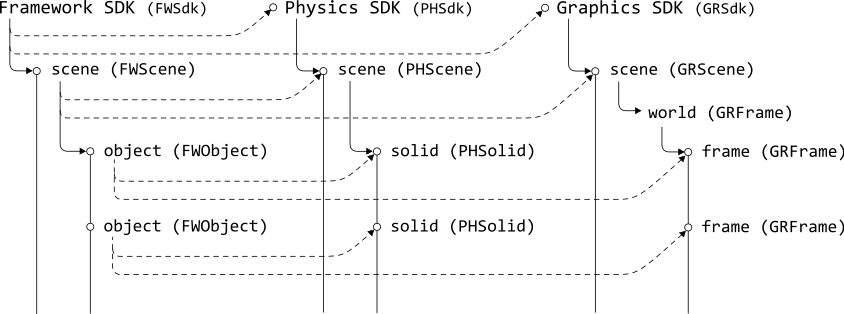
\includegraphics[width=.9\hsize]{fig/fwscene.eps}
\end{center}
\caption{Data structure of Framework, Physics and Graphics modules}
\label{fig_fwscene}
\end{figure}

\index{FWScene}
\index{FWObject}
Framework\KLUDGE モジュールの主な機能の1\KLUDGE つにPhysics\KLUDGE シーンとGraphics\KLUDGE シーンの同期があります.
Fig.\,\ref{fig_fwscene}\KLUDGE に3\KLUDGE つのモジュールのSDK\KLUDGE とシーンの関係を示します.
\texttt{FWSdk}\KLUDGE は任意の数のシーン(\texttt{FWScene}\KLUDGE クラス)を保持します.
\KLUDGE また,シーンは任意の数のオブジェクト(\texttt{FWObject}\KLUDGE クラス)を保持します.
Fig.\,\ref{fig_fwscene}\KLUDGE に示すように,
\KLUDGE オブジェクトはPhysics\KLUDGE モジュールの剛体とGraphics\KLUDGE モジュールのトップフレームを一対一に対応づけます.
\KLUDGE ここでトップフレームとはワールドフレームの直下にあるフレームのことです.
\KLUDGE 物理シミュレーションにより計算される剛体の運動をフレームの座標変換に反映させることで,
\KLUDGE シミュレーションの様子をGraphics\KLUDGE モジュールの機能を利用して可視化することができるようになります.

\KLUDGE シーン作成に関する\texttt{FWSdk}\KLUDGE の関数を以下に示します.

\noindent
\begin{tabular}{p{1.0\hsize}}
\\
\texttt{HITrackballIf}														\\ \midrule
\texttt{FWSceneIf* CreateScene(const PHSceneDesc\&, const GRSceneDesc\&)}	\\
\KLUDGE シーンを作成する.															\\
\\
\texttt{int NScene()}	\\
\KLUDGE シーンの数を取得する	\\
\\
\texttt{FWSceneIf* GetScene(int i)}	\\
\texttt{i}\KLUDGE 番目のシーンを取得する.	\\
\\
\texttt{void MergeScene(FWSceneIf* scene0, FWSceneIf* scene1)}	\\
\texttt{scene1}\KLUDGE の子オブジェクトを\texttt{scene0}\KLUDGE に移す.		\\
\\
\end{tabular}

\KLUDGE シーンを作成するには以下のようにします.
\begin{sourcecode}
FWSceneIf* fwScene = fwSdk->CreateScene();
\end{sourcecode}
\texttt{FWScene}\KLUDGE を作成すると,同時に\texttt{PHScene}\KLUDGE と\texttt{GRScene}\KLUDGE も作成され,\texttt{FWScene}\KLUDGE とリンクされます.
\texttt{CreateScene}\KLUDGE にディスクリプタを指定することもできます.
\texttt{NScene}\KLUDGE は作成したシーンの数を返します.

%\KLUDGE シーンはいくつでも作成できますが,その中の1\KLUDGE つのシーンが選択された状態にあります.
%\KLUDGE 選択されたシーンをカレントシーンと呼びます.
%\KLUDGE 新しく作成されたシーンはカレントシーンとなります.
%\KLUDGE 選択を切り替えるには\texttt{SwitchScene}\KLUDGE を使います.

\KLUDGE シーンを取得するには\texttt{GetScene}\KLUDGE を使います.
\texttt{GetScene}\KLUDGE に指定する整数は作成された順番にシーンに与えられる通し番号です.
%\KLUDGE 引数を省略するとカレントシーンが返されます.
\begin{sourcecode}
fwSdk->CreateScene();               // create two scenes
fwSdk->CreateScene();
FWSceneIf *fwScene0, *fwScene1;
fwScene0 = fwSdk->GetScene(0);      // get 1st scene
fwScene1 = fwSdk->GetScene(1);      // get 2nd scene
\end{sourcecode}

\texttt{MergeScene}\KLUDGE を使うと2\KLUDGE つのシーンを統合して1\KLUDGE つのシーンにできます.
\begin{sourcecode}
fwSdk->MergeScene(fwScene0, fwScene1);
\end{sourcecode}
\KLUDGE 上のコードでは\texttt{scene1}\KLUDGE が持つ\texttt{FWObject}\KLUDGE が\texttt{scene0}\KLUDGE に移され,同時にシーンが参照する
\texttt{PHScene}\KLUDGE と\texttt{GRScene}\KLUDGE に関してもそれぞれの\texttt{MergeScene}\KLUDGE 関数により統合が行われます.

\KLUDGE 次に,\texttt{FWScene}\KLUDGE の基本機能を以下に示します.

\noindent
\begin{tabular}{p{.6\hsize}p{.3\hsize}}
\\
\texttt{FWSceneIf}													\\ \midrule
\texttt{void SetPHScene(PHSceneIf*)}	& Physics\KLUDGE シーンの設定		\\
\texttt{PHSceneIf* GetPHScene()}		& Physics\KLUDGE シーンの取得		\\
\texttt{void SetGRScene(GRSceneIf*)}	& Graphics\KLUDGE シーンの設定		\\
\texttt{GRSceneIf* GetGRScene()}		& Graphics\KLUDGE シーンの取得		\\
\texttt{FWObjectIf* CreateFWObject()}	& \KLUDGE オブジェクトの作成		\\
\texttt{int NObject()const}				& \KLUDGE オブジェクトの数			\\
\texttt{FWObjectIf** GetObjects()}		& \KLUDGE オブジェクト配列の取得	\\
\texttt{void Sync(bool)}				& \KLUDGE 同期						\\
\\
\end{tabular}

\texttt{[Set|Get][PH|GR]Scene}\KLUDGE 関数はシーンに割り当てられた\texttt{PHScene}\KLUDGE や\texttt{GRScene}\KLUDGE を取得したり,別のシーンを割り当てたりするのに使用します.

\texttt{CreateFWObject}\KLUDGE 関数は\texttt{FWObject}\KLUDGE オブジェクトを作成します.
\KLUDGE このとき,新たに作成された\texttt{FWObject}\KLUDGE には\texttt{PHSolid}\KLUDGE および\texttt{GRFrame}\KLUDGE は割り当てられていない状態になっているので注意してください.
\KLUDGE これらも同時に作成するには,以下のコードを1\KLUDGE セットで実行します.

\begin{sourcecode}
FWObjectIf* fwObj = fwScene->CreateFWObject();
fwObj->SetPHSolid(fwScene->GetPHScene()->CreateSolid());
fwObj->SetGRFrame(
    fwScene->GetGRScene()->CreateVisual(GRFrameDesc())->Cast);
\end{sourcecode}

\texttt{Sync}\KLUDGE 関数は\texttt{PHScene}\KLUDGE と\texttt{GRScene}\KLUDGE の同期に用います.
\begin{sourcecode}
fwScene->Sync(true);
\end{sourcecode}
\KLUDGE とすると,このシーンが参照する\texttt{PHScene}\KLUDGE 中の剛体の位置と向きが,
\KLUDGE 同じくこのシーンが参照する\texttt{GRScene}\KLUDGE 中のトップフレームの位置と向きに反映されます.
\KLUDGE このときの剛体とトップフレームとの対応関係は\texttt{FWObject}\KLUDGE により定義されます.

\KLUDGE 逆に
\begin{sourcecode}
fwScene->Sync(false);
\end{sourcecode}
\KLUDGE とすると,同様のメカニズムで各トップフレームの位置と向きが対応する剛体に反映されます.

\section{\KLUDGE シーンのロードとセーブ}

FileIO\KLUDGE モジュールを利用してシーンをロード,セーブするための関数が用意されています.
\KLUDGE まずロードには以下の関数を用います.

\noindent
\begin{tabular}{p{1.0\hsize}}
\\
\texttt{FWSdkIf}														\\ \midrule
\texttt{bool LoadScene(UTString path, ImportIf* imp, const IfInfo* ii, ObjectIfs* objs)}	\\
\KLUDGE シーンをロードする.		\\
\\
\end{tabular}

\texttt{path}\KLUDGE はロードするファイルへのパスを格納した文字列です.
\texttt{imp}\KLUDGE にはインポート情報を格納するための\texttt{Import}\KLUDGE オブジェクトを与えます.
\KLUDGE インポート情報を記憶する必要のない場合は\texttt{NULL}\KLUDGE で構いません.
\texttt{ii}\KLUDGE はロードするファイルの種類を明示するための型情報です.
\texttt{NULL}\KLUDGE を指定するとパスの拡張子から自動判別されます.
\texttt{objs}\KLUDGE はロードによって作成されるオブジェクトツリーの親オブジェクトを格納した配列です.

\KLUDGE ロードに成功すると\texttt{true}\KLUDGE ,失敗すると\texttt{false}\KLUDGE が返されます.
\KLUDGE ロードされたシーンは\texttt{FWSdk}\KLUDGE のシーン配列の末尾に加えられます.

\KLUDGE 次に,シーンをセーブするには以下の関数を使います.

\noindent
\begin{tabular}{p{1.0\hsize}}
\\
\texttt{FWSdkIf}														\\ \midrule
\texttt{bool SaveScene(UTString path, ImportIf* imp, const IfInfo* ii, ObjectIfs* objs)}	\\
\KLUDGE シーンをセーブする.		\\
\\
\end{tabular}

\KLUDGE 引数の意味は\texttt{LoadScene}\KLUDGE と同様です.
\texttt{imp}\KLUDGE にはロード時に記憶したインポート情報を与えます.
\KLUDGE 省略するとシーン全体が単一のファイルにセーブされます.

\KLUDGE セーブに成功すると\texttt{true}\KLUDGE ,失敗すると\texttt{false}\KLUDGE が返されます.


\section{Framework \KLUDGE オブジェクト}

\texttt{FWObject}\KLUDGE は\texttt{PHSolid}\KLUDGE と\texttt{GRFrame}\KLUDGE の橋渡しが主な役割ですので,それ自体はそれほど多くの機能を持っていません.


\section{\KLUDGE アプリケーションクラス}

\index{FWApp}
Springhead\KLUDGE を利用するアプリケーションの作成を容易にするために,アプリケーションクラス\texttt{FWApp}\KLUDGE が用意されています.
\ref{sec_create_application}\KLUDGE に\texttt{FWApp}\KLUDGE を使って簡単なアプリケーションを作成する方法について説明しましたのでそちらも合わせて参考にしてください.

\KLUDGE 冒頭で説明した通り,Springhead\KLUDGE のほとんどのオブジェクトは,親オブジェクトの\texttt{Create}\KLUDGE 系関数を使って作成しますが,
\texttt{FWApp}\KLUDGE は例外的に,C++\KLUDGE のクラス継承を用いてユーザのアプリケーションクラスを定義する方法をとります.
\KLUDGE この方が仮想関数によって動作のカスタマイズがフレキシブルに行えるからです.

\KLUDGE 以下では\texttt{FWApp}\KLUDGE の機能やユーザが実装すべき仮想関数について順に見ていきます.

\subsection*{\KLUDGE 初期化}

\texttt{FWApp}\KLUDGE の初期化処理は仮想関数\texttt{Init}\KLUDGE で行います.

\noindent
\begin{tabular}{p{.7\hsize}p{.2\hsize}}
\\
\texttt{FWApp}											\\ \midrule
\texttt{virtual void Init(int argc, char* argv[])}	&	\\
\\
\end{tabular}

\KLUDGE 以下に\texttt{Init}\KLUDGE 関数のデフォルトの実装を示します.

\begin{sourcecode}
void FWApp::Init(int argc, char* argv[]){
    // create SDK
    CreateSdk();
    // create a single scene
    GetSdk()->CreateScene();
    // initialize window manager
    GRInit(argc, argv);
    // create main window
    CreateWin();
    // create timer
    CreateTimer();
}
\end{sourcecode}
\KLUDGE はじめに
\begin{sourcecode}
    CreateSdk();
\end{sourcecode}
\KLUDGE でSDK\KLUDGE を作成します.
\KLUDGE つぎに
\begin{sourcecode}
    GRInit(argc, argv);
\end{sourcecode}
\KLUDGE でウィンドウマネジャが作成されます.
\KLUDGE デフォルトではGLUT\KLUDGE を用いるウィンドウマネジャが作成されます.
\KLUDGE さらに
\begin{sourcecode}
    GetSdk()->CreateScene();
\end{sourcecode}
\KLUDGE で\texttt{FWScene}\KLUDGE を1\KLUDGE つ作成します.
\KLUDGE つづいて
\begin{sourcecode}
    CreateWin();
\end{sourcecode}
\KLUDGE でメインウィンドウを作成します.
\KLUDGE 最後に
\begin{sourcecode}
    CreateTimer();
\end{sourcecode}
\KLUDGE でタイマを作成します.

\KLUDGE この基本処理に追加してなんらかの処理を行う場合は
\begin{sourcecode}
virtual void Init(int argc = 0, char* argv[] = 0){
    // select GLUI window manager
    SetGRAdaptee(TypeGLUI);

    // call base Init
    FWApp::Init(argc, argv);

    // do extra initialization here


}
\end{sourcecode}
\KLUDGE のように,\texttt{FWApp:Init}\KLUDGE を実行してから追加の処理を行うのが良いでしょう.
\KLUDGE 一方,以下に挙げるようなカスタマイズが必要な場合は\texttt{Init}\KLUDGE 関数の処理全体を派生クラスに記述する必要があります.
\begin{itemize}
\item \KLUDGE シーン生成をカスタマイズしたい
\item \KLUDGE ウィンドウの初期サイズやタイトルを変更したい
\item \KLUDGE 異なる種類のタイマが使いたい
\end{itemize}
\KLUDGE この場合は,上に載せた\texttt{Init}\KLUDGE のデフォルト処理をもとに必要な部分に修正を加えるのが良いでしょう.

\KLUDGE プログラムの全体の構造は通常以下のようになります.

\begin{sourcecode}
MyApp app;

int main(int argc, char* argv[]){
    app.Init(argc, argv);
    app.StartMainLoop();
    return 0;
}
\end{sourcecode}

\KLUDGE ここで\texttt{MyApp}\KLUDGE はユーザが定義した\texttt{FWApp}\KLUDGE の派生クラスです(もちろん他の名前でも構いません).
\texttt{MyApp}\KLUDGE のインスタンスをグローバル変数として定義し,
\texttt{main}\KLUDGE 関数で\texttt{Init}\KLUDGE ,\texttt{StartMainLoop}\KLUDGE を順次実行します.
\texttt{StartMainLoop}\KLUDGE 関数はアプリケーションのメインループを開始します.


\subsection*{\KLUDGE タイマ}

\KLUDGE タイマの作成には\texttt{CreateTimer}\KLUDGE 関数を使います.
\KLUDGE 通常,\texttt{CreateTimer}\KLUDGE は\texttt{Init}\KLUDGE の中で呼びます.

\noindent
\begin{tabular}{p{.7\hsize}p{.2\hsize}}
\\
\texttt{FWApp}												\\ \midrule
\texttt{UTTimerIf* CreateTimer(UTTimerIf::Mode mode)}	&	\\
\\
\end{tabular}

\KLUDGE 引数\texttt{mode}\KLUDGE に指定できる値は\texttt{UTTimer}\KLUDGE の\texttt{SetMode}\KLUDGE と同じです.
\ref{sec_uttimer}\KLUDGE 節を参照してください.
\KLUDGE 戻り値として\texttt{UTTimer}\KLUDGE のインタフェースが返されます.
\KLUDGE 周期などの設定はこのインタフェースを介して行います.

\KLUDGE シミュレーション用と描画用に2\KLUDGE つのタイマを作成する例を以下に示します.
\begin{sourcecode}
UTTimerIf *timerSim, *timerDraw;
timerSim = CreateTimer(MULTIMEDIA);
timerSim->SetInterval(10);
timerDraw = CreateTimer(FRAMEWORK);
timerDraw->SetInterval(50);
\end{sourcecode}
\KLUDGE この例ではシミュレーション用には周期を$10$[ms]\KLUDGE のマルチメディアタイマを使い,
\KLUDGE 描画用には周期$50$[ms]\KLUDGE のフレームワークタイマ(GLUT\KLUDGE タイマ)を使っています.

\KLUDGE タイマを始動すると,周期ごとに以下の仮想関数が呼ばれます.

\noindent
\begin{tabular}{p{.7\hsize}p{.2\hsize}}
\\
\texttt{FWApp}								\\ \midrule
\texttt{virtual void TimerFunc(int id)}	&	\\
\\
\end{tabular}
\KLUDGE タイマの判別は引数$id$\KLUDGE で行います.

\texttt{TimerFunc}\KLUDGE のデフォルトの振る舞いでは,
\KLUDGE カレントウィンドウのシーンの\texttt{Step}\KLUDGE を呼び,つぎに\texttt{PostRedisplay}\KLUDGE で再描画要求を発行します
\KLUDGE (その結果,直後に\texttt{Display}\KLUDGE 関数が呼び出されます).
\KLUDGE この振る舞いをカスタマイズしたい場合は\texttt{TimerFunc}\KLUDGE 関数をオーバライドします.
\begin{sourcecode}
void TimerFunc(int id){
    // proceed simulation of scene attached to current window
    if(id == timerSim->GetID()){
        GetCurrentWin()->GetScene()->Step();
    }
    // generate redisplay request
    else if(id == timerDraw->GetID()){
        PostRedisplay();
    }
}
\end{sourcecode}
\KLUDGE この例ではシミュレーションと描画に異なる2\KLUDGE つのタイマを使用しています.

\subsection*{\KLUDGE 描画}

\KLUDGE 描画処理は次の仮想関数で行います.

\noindent
\begin{tabular}{p{.7\hsize}p{.2\hsize}}
\\
\texttt{FWApp}						\\ \midrule
\texttt{virtual void Display()}	&	\\
\\
\end{tabular}

\texttt{Display}\KLUDGE は描画要求が発行されたときに呼び出されます.
\KLUDGE 描画要求は\texttt{PostRedisplay}\KLUDGE 関数で行います.

\noindent
\begin{tabular}{p{.7\hsize}p{.2\hsize}}
\\
\texttt{FWApp}							\\ \midrule
\texttt{virtual void PostRedisplay()}	&	\\
\\
\end{tabular}

\texttt{Display}\KLUDGE 関数のデフォルトの振る舞いではカレントウィンドウの\texttt{Display}\KLUDGE 関数が呼ばれます.

\subsection*{\KLUDGE キーボード・マウスイベント}

\texttt{FWApp}\KLUDGE は各ウィンドウに関連付けられた仮想キーボード・マウスデバイス\texttt{DVKeyMouse}\KLUDGE にコールバック登録されています.
\KLUDGE したがって以下の仮想関数をオーバライドすることでキーボード・マウスイベントを処理できます.

\noindent
\begin{tabular}{p{1.0\hsize}}
\\
\texttt{FWApp}							\\ \midrule
\texttt{virtual bool OnMouse(int button, int state, int x, int y)}	\\
\texttt{virtual bool OnDoubleClick(int button, int x, int y)}	\\
\texttt{virtual bool OnMouseMove(int state, int x, int y, int zdelta)}	\\
\texttt{virtual bool OnKey(int state, int key, int x, int y)}	\\
\\
\end{tabular}

\KLUDGE 各イベントハンドラの詳細については\ref{sec_hi_keymouse}\KLUDGE 節を参照して下さい.

\section{\KLUDGE ウィンドウ}

\KLUDGE ウィンドウやその他のGUI\KLUDGE コントロールの作成もFramework\KLUDGE によってサポートされています.
\KLUDGE すでに述べてきたとおり,\texttt{FWApp}\KLUDGE はトップレベルウィンドウの配列を持ちます.




\section{Framework\KLUDGE を用いたシミュレーションと描画}

Framework\KLUDGE モジュールを介して物理シミュレーションを行うには以下の関数を使います.

\noindent
\begin{tabular}{p{.7\hsize}p{.2\hsize}}
\\
\texttt{FWSdkIf}			\\ \midrule
\texttt{void Step()}	& 	\\
\end{tabular}
\noindent

\texttt{FWSdk}\KLUDGE の\texttt{Step}\KLUDGE はアクティブシーンの\texttt{Step}\KLUDGE を呼びます.
\KLUDGE したがって\texttt{GetScene()->Step()}\KLUDGE と等価です.
\KLUDGE 一方\texttt{FWScene}\KLUDGE の\texttt{Step}\KLUDGE は,保持している\texttt{PHScene}\KLUDGE の\texttt{Step}\KLUDGE を呼びます.
\KLUDGE したがって\texttt{GetPHScene()->Step()}\KLUDGE と等価です.
\KLUDGE 両方とも薄いラッパー関数ですが,ユーザのタイプ回数節約のために用意されています.

Framework\KLUDGE を用いた描画には2\KLUDGE 通りの方法があります.
1\KLUDGE つはGraphics\KLUDGE のシーングラフを用いる方法,もう1\KLUDGE つはPhysics\KLUDGE シーンを直接描画する方法です.
\KLUDGE 後者はデバッグ描画とも呼ばれています.

\noindent
\begin{tabular}{p{.7\hsize}p{.2\hsize}}
\\
\texttt{FWSdkIf}						\\ \midrule
\texttt{void Draw()}				&	\\
\texttt{void SetDebugMode(bool)}	& 	\\
\texttt{bool GetDebugMode()}		&	\\
\\
\end{tabular}

\texttt{Draw}\KLUDGE 関数は描画モードに応じた描画処理を行います.
\texttt{Draw}\KLUDGE は通常アプリケーションの描画ハンドラから呼び出します.
\texttt{[Set|Get]DebugMode}\KLUDGE は通常描画モード(\texttt{false})\KLUDGE とデバッグ描画モード(\texttt{true})\KLUDGE を切り替えます.

\KLUDGE 通常描画モードにおいて\texttt{Draw}\KLUDGE 関数を呼ぶと,
\KLUDGE はじめにアクティブシーンについて\texttt{Sync(true)}\KLUDGE が呼ばれ,剛体の状態がシーングラフに反映されます.
\KLUDGE 次にアクティブシーンが参照する\texttt{GRScene}\KLUDGE の\texttt{Render}\KLUDGE 関数が呼ばれ,シーングラフが描画されます.
\KLUDGE この方法ではシーングラフが持つライトやテクスチャなどの情報を最大限利用してフォトリアリスティックな描画が可能です.
\KLUDGE その反面,物理シミュレーションが主目的である場合にはシーングラフの構築という付加的なコストを支払わなければならないというデメリットもあります.

\KLUDGE デバッグ描画については次節で説明します.

\section{\KLUDGE デバッグ描画}

\KLUDGE デバッグ描画モードでは\texttt{PHScene}\KLUDGE の情報だけを用いて描画が行われるので,シーングラフ構築の手間が省けます.
\KLUDGE また,剛体に加わる力などの物理シミュレーションに関する情報を可視化することができます.
\KLUDGE 一方で,予約色しか使えないなど,描画の自由度には一定の制約が生じます.

\KLUDGE デバッグ描画モードでは\texttt{FWScene}\KLUDGE の\texttt{DrawPHScene}\KLUDGE 関数により描画処理が行われます.

\noindent
\begin{tabular}{p{.7\hsize}p{.2\hsize}}
\\
\texttt{FWSceneIf}									\\ \midrule
\texttt{void DrawPHScene(GRRenderIf* render)}	&	\\
\\
\end{tabular}

\texttt{DrawPHScene}\KLUDGE は,各剛体に割り当てられている衝突判定形状,座標軸,作用している力,接触断面などを描画します.
\KLUDGE 項目別に描画を行ったり,描画色を設定するには後述する描画制御関数を用います.

\subsection*{\KLUDGE デバッグ描画時のカメラとライト}

\KLUDGE デバッグ描画においてもカメラの情報は\texttt{GRScene}\KLUDGE が参照されます.
\KLUDGE もし\texttt{GRScene}\KLUDGE がカメラを保有している場合はそのカメラの\texttt{Render}\KLUDGE が呼ばれ,視点と投影変換が設定されます.
\texttt{GRScene}\KLUDGE がカメラを持たない場合は手動で設定する必要があります.

\KLUDGE ライトについては,もし外部でレンダラに対してライト設定がされている場合はその設定が優先され,
\KLUDGE レンダラが1\KLUDGE つもライトを持たない場合は内部でデフォルトライトが設定されます.

\subsection*{\KLUDGE 個別の描画}

\KLUDGE 以下の関数は\texttt{DrawPHScene}\KLUDGE から呼び出されますが,ユーザが個別に呼び出すこともできます.

\noindent
\begin{tabular}{p{.7\hsize}p{.2\hsize}}
\\
\texttt{FWSceneIf}												\\ \midrule
\texttt{void DrawSolid(GRRenderIf*, PHSolidIf*, bool)}		&	\KLUDGE 剛体を描画\\
\texttt{void DrawShape(GRRenderIf*, CDShapeIf*, bool)}		&	\KLUDGE 形状を描画\\
\texttt{void DrawConstraint(GRRenderIf*, PHConstraintIf*)}	&	\KLUDGE 拘束を描画\\
\texttt{void DrawContact(GRRenderIf*, PHContactPointIf*)}	&	\KLUDGE 接触を描画\\
\texttt{void DrawIK(GRRenderIf*, PHIKEngineIf*)}			&	IK\KLUDGE 情報を描画\\
\\
\end{tabular}

\subsection*{\KLUDGE 描画制御}

\KLUDGE 以下の関数は描画のOn/Off\KLUDGE を切り替えます.

\noindent
\begin{tabular}{p{.8\hsize}p{.1\hsize}}
\\
\texttt{FWSceneIf}													\\ \midrule
\texttt{void SetRenderMode(bool solid, bool wire)}					&	\\
\texttt{void EnableRender(ObjectIf* obj, bool enable)}				&	\\
\texttt{void EnableRenderAxis(bool world, bool solid, bool con)}	&	\\
\texttt{void EnableRenderForce(bool solid, bool con)}				&	\\
\texttt{void EnableRenderContact(bool enable)}						&	\\
\texttt{void EnableRenderGrid(bool x, bool y, bool z)}				&	\\
\texttt{void EnableRenderIK(bool enable)}							&	\\
\\
\end{tabular}

\texttt{SetRenderMode}\KLUDGE はソリッド描画(面を塗りつぶす)とワイヤフレーム描画(面の輪郭)のOn/Off\KLUDGE を切り替えます.

\texttt{EnableRender}\KLUDGE は指定したオブジェクトの描画のOn/Off\KLUDGE を切り替えます.
\KLUDGE 項目ではなくオブジェクトレベルで描画制御したい場合に便利です.
\texttt{obj}\KLUDGE に指定できるのは剛体(\texttt{PHSolidIf*})\KLUDGE か拘束(\texttt{PHConstraintIf*})\KLUDGE です.

\texttt{EnableRenderAxis}\KLUDGE は項目別に座標軸の描画を設定します.
\texttt{world}\KLUDGE はワールド座標軸,\texttt{solid}\KLUDGE は剛体,\texttt{con}\KLUDGE は拘束の座標軸です.

\texttt{EnableRenderForce}\KLUDGE は力とモーメントの描画を設定します.
\texttt{solid}\KLUDGE は剛体に加わる力(ただし外力のみで拘束力は除く),\texttt{con}\KLUDGE は拘束力です.

\texttt{EnableRenderGrid}\KLUDGE は各軸に関してグリッドの描画を設定します.

\texttt{EnableRenderIK}\KLUDGE はIK\KLUDGE 情報の描画を設定します.

\KLUDGE 以下の関数は描画属性を指定するのに使います.

\noindent
\begin{tabular}{p{.8\hsize}p{.1\hsize}}
\\
\texttt{FWSceneIf}																\\ \midrule
\texttt{void SetSolidMaterial(int mat, PHSolidIf* solid)}						&	\\
\texttt{void SetWireMaterial (int mat, PHSolidIf* solid)}						&	\\
\texttt{void SetAxisMaterial(int matX, int matY, int matZ)}						&	\\
\texttt{void SetAxisScale(float world, float solid, float con)}					&	\\
\texttt{void SetAxisStyle(int style)}											&	\\
\texttt{void SetForceMaterial(int matForce, int matMoment)}						&	\\
\texttt{void SetForceScale(float scaleForce, float scaleMoment)}				&	\\
\texttt{void SetContactMaterial(int mat)}										&	\\
\texttt{void SetGridOption(char axis, float offset, float size, int slice)}		&	\\
\texttt{void SetGridMaterial(int matX, int matY, int matZ)}						&	\\
\texttt{void SetIKMaterial(int mat)}											&	\\
\texttt{void SetIKScale(float scale)}											&	\\
\\
\end{tabular}

\texttt{SetSolidMaterial}\KLUDGE は指定した剛体のソリッド描画色を指定します.
\texttt{mat}\KLUDGE に指定できる値は\ref{sec_grmaterial}\KLUDGE 節で述べた予約色です.
\texttt{solid}\KLUDGE に\texttt{NULL}\KLUDGE を指定するとすべての剛体の色が指定された値になります.
\texttt{SetWireMaterial}\KLUDGE は同様に剛体のワイヤフレーム描画色を指定します.

\texttt{SetAxisMaterial}\KLUDGE は座標軸の色をx, y, z\KLUDGE 個別に指定します.
\texttt{SetAxisScale}\KLUDGE は座標軸の縮尺を指定します.
\texttt{SetAxisStyle}\KLUDGE は座標軸のスタイルを指定します.

\texttt{SetForceMaterial}\KLUDGE ,\texttt{SetForceScale}\KLUDGE はそれぞれ力(並進力とモーメント)の描画色と縮尺を指定します.

\texttt{SetContactMaterial}\KLUDGE は接触断面の描画色を指定します.

\texttt{SetGridOption}\KLUDGE はグリッドのオプションを指定します.
\texttt{SetGridMaterial}\KLUDGE はグリッドの描画色を指定します.

\texttt{SetIKMaterial}\KLUDGE ,\texttt{SetIKScale}\KLUDGE はIK\KLUDGE 情報の描画色と縮尺を指定します.


\section{\KLUDGE 力覚インタラクションのためのアプリケーション}
Springhead2\KLUDGE にはシーンとの力覚インタラクションのためのエンジン\texttt{PHHapticEngine}\KLUDGE が含まれています.
\KLUDGE ここでは力覚インタラクションのためのアプリケーションの作成方法について説明します.
\KLUDGE まずは,通常の\texttt{Framework}\KLUDGE アプリケーションの作成と同様に,ひな形クラスである\texttt{FWApp}\KLUDGE を継承してアプリケーションを
\KLUDGE 作成します.
\KLUDGE そして,\texttt{Init}\KLUDGE 関数内で力覚インタラクションを有効化と,力覚インタラクションシステムのモードを設定します.
\begin{sourcecode}
	// given PHSceneIf* phScene,
    phScene->GetHapticEngine()->EnableHapticEngine(true);
    phScene->GetHapticEngine()->
    SetHapticEngineMode(PHHapticEngineDesc::MULTI_THREAD);
\end{sourcecode}
\KLUDGE 力覚インタラクションシステムのモードは
\KLUDGE シングルスレッドアプリケーションのための\texttt{SINGLE\_THREAD}\KLUDGE ,
\KLUDGE マルチメディアアプリケーションのための\texttt{MULTI\_THREAD}\KLUDGE ,局所シミュレーションを利用した\texttt{LOCAL\_DYNAMICS}\KLUDGE の3\KLUDGE 種類があります.
\KLUDGE 標準では\texttt{MULTI\_THREAD}\KLUDGE が設定されています.
\texttt{MULTI\_THREAD}\KLUDGE ,\texttt{LOCAL\_DYNAMICS}\KLUDGE のモードはマルチスレッドを利用したアプリケーションとなり,
\KLUDGE 物理シミュレーションを実行する物理スレッド,力覚レンダリングを実行する力覚スレッドが並列に動きます.
\KLUDGE そのため,それぞれのスレッドをコールバックするためにタイマを設定し直す必要があります.
\clearpage

\begin{sourcecode}
	// given PHSceneIf* phScene,
	int physicsTimerID, hapticTimerID // 各タイマのID
	// FWApp::TimerFuncをオーバライドしたコールバック関数
	void MyApp::TimerFunc(int id){
        if(hapticTimerID == id){
            // 力覚スレッドのコールバック
            phScene->StepHapticLoop();	
        }else{
            // 物理スレッドのコールバック
            phScene->GetHapticEngine()->StepPhysicsSimulation();	
            PostRedisplay();	// 描画
        }	
	}	
\end{sourcecode}


\KLUDGE 次にユーザがオブジェクトとインタラクションするためのポインタ,力覚ポインタ\texttt{PHHapticPointer}\KLUDGE を作ります.
\KLUDGE そして,どのインタフェースと結合するのかを設定します.
\texttt{PHHapticPointer}\KLUDGE は\texttt{PHScene}\KLUDGE から作ることができます.
\texttt{PHHapticPointer}\KLUDGE は\texttt{PHSolid}\KLUDGE を継承したクラスで\texttt{PHSolid}\KLUDGE の関数を利用して,
\KLUDGE 質量,慣性テンソル,形状などを合わせて設定します.
\KLUDGE 例えばSpidar-G6\KLUDGE と接続する場合には,

\begin{sourcecode}
	// given PHSceneIf* phScene,
	// given HISpidarIf* spg,
    PHHapticPointerIf* pointer = phScene->CreateHapticPointer();
    /*
        質量,慣性テンソル,形状などを設定する
    */
    pointer->SetHumanInterface(spg);
\end{sourcecode}
\KLUDGE とします.
\KLUDGE さらにPHHapticPointer\KLUDGE について以下の関数を用いて,力覚提示のためのパラメータを設定します.

\noindent
\begin{tabular}{p{.8\hsize}p{.1\hsize}}
\\
\texttt{PHHapticPointerIf}													\\ \midrule
\texttt{void SetHumanInterface(HIBaseIf* interface)}						&	\\
\texttt{void SetDefaultPose(Posed pose)}									&	\\
\texttt{void SetPosScale(double scale)}										&	\\
\texttt{void SetReflexSpring(float s)}										&	\\
\texttt{void SetReflexDamper(float s)}										&	\\
\texttt{void EnableFriction(bool b)}										&	\\
\texttt{void EnableVibration(bool b)}										&	\\
\texttt{void SetLocalRange(float s)}										&	\\
\texttt{void SetHapticRenderMode(PHHapticPointerDesc::HapticRenderMode m )}	&	\\
\\
\end{tabular}

\texttt{SetHumanInterface}\KLUDGE は力覚ポインタにヒューマンインタフェースを割り当てます.
\texttt{SetDefaultPose}\KLUDGE はシーン内での力覚ポインタの初期位置を指定します.
\texttt{SetPosScale}\KLUDGE はシーン内での力覚ポインタの可動スケールを指定します.
\texttt{SetReflexSpring}\KLUDGE は力覚レンダリング(反力計算)のためのバネ係数値を設定します.
\texttt{SetReflexDamper}\KLUDGE は力覚レンダリングのためのダンパ係数値を設定します.
\texttt{EnableFriction}\KLUDGE は力覚ポインタの摩擦力提示を有効化します.
\texttt{EnableVibration}\KLUDGE は力覚ポインタの振動提示を有効化します.
\texttt{SetLocalRange}\KLUDGE は局所シミュレーションシステムを使用時の局所シミュレーション範囲を指定します.
\texttt{SetHapticRenderMode}\KLUDGE は力覚レンダリングのモードを指定します.

\KLUDGE 最後の\texttt{SetHapticRenderMode}\KLUDGE には\texttt{PENALTY}\KLUDGE ,\texttt{CONSTRAINT}\KLUDGE のモードがあります.
\texttt{PENALTY}\KLUDGE は力覚ポインタが剛体に接触した時の各接触点の侵入量とバネダンパ係数を乗じたものを足しあわせたものが
\KLUDGE 反力として計算され,インタフェースから出力されます.\texttt{CONSTRAINT}\KLUDGE は力覚ポインタが剛体に侵入していない状態(プロキシ)を
\KLUDGE 求め,力覚ポインタとプロキシの距離の差分にバネダンパ係数を乗じたものを反力として計算します.
